%=======================02-713 LaTeX template, following the 15-210 template==================
%
% You don't need to use LaTeX or this template, but you must turn your homework in as
% a typeset PDF somehow.
%
% How to use:
%    1. Update your information in section "A" below
%    2. Write your answers in section "B" below. Precede answers for all 
%       parts of a question with the command "\question{n}{desc}" where n is
%       the question number and "desc" is a short, one-line description of 
%       the problem. There is no need to restate the problem.
%    3. If a question has multiple parts, precede the answer to part x with the
%       command "\part{x}".
%    4. If a problem asks you to design an algorithm, use the commands
%       \algorithm, \correctness, \runtime to precede your discussion of the 
%       description of the algorithm, its correctness, and its running time, respectively.
%    5. You can include graphics by using the command \includegraphics{FILENAME}
%
\documentclass[11pt]{article}
\usepackage{amsmath,amssymb,amsthm}
\usepackage{graphicx}
\usepackage[margin=1in]{geometry}
\usepackage{fancyhdr}
\setlength{\parindent}{0pt}
\setlength{\parskip}{5pt plus 1pt}
\setlength{\headheight}{13.6pt}
\newcommand\question[2]{\vspace{.25in}\hrule\textbf{#1: #2}\vspace{.5em}\hrule\vspace{.10in}}
\renewcommand\part[1]{\vspace{.10in}\textbf{(#1)}\par}
\newcommand\algorithm{\vspace{.10in}\textbf{Algorithm: }}
\newcommand\correctness{\vspace{.10in}\textbf{Correctness: }}
\newcommand\runtime{\vspace{.10in}\textbf{Running time: }}
\pagestyle{fancyplain}
\lhead{\textbf{\NAME}}
\chead{\textbf{{\COURSE} HW\HWNUM}}
\rhead{\today}
\begin{document}\raggedright
%Section A==============Change the values below to match your information==================
\newcommand\NAME{Eric Altenburg}	% your name
\newcommand\COURSE{MA-331} 		% the course number
\newcommand\HWNUM{7}              		% the homework number
%Section B==============Put your answers to the questions below here=======================

% no need to restate the problem --- the graders know which problem is which,
% but replacing "The First Problem" with a short phrase will help you remember
% which problem this is when you read over your homeworks to study.

\begin{center}
	\textit{Pledge: I pledge my honor that I have abided by the Stevens Honor System.} - \textbf{\NAME}
\end{center}


\question{10.32}{Page 606}
	\part{a}
		Numerical data for IBI:\par
		
		\begin{center}
		\begin{tabular}{cccccccc}
			n & Mean & St. Deviation & Minimum & Q1 & Median & Q3 & Maximum\\
			49 & 65.94 & 18.28 & 29 & 54.50 & 71 & 82 & 91\\
		\end{tabular}\par
		\end{center}
		Histogram for IBI:\par
		
		\begin{center}
		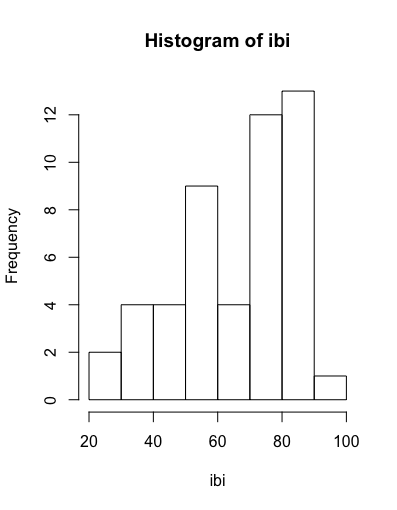
\includegraphics[scale=0.5]{images/ibihist.png}
		\end{center}\par
		Based on this, it is left-skewed.\par
		
		\begin{center}
		\begin{tabular}{cccccccc}
			n & Mean & St. Deviation & Minimum & Q1 & Median & Q3 & Maximum\\
			49 & 28.29 & 17.71 & 2 & 15 & 26 & 36.5 & 70\\
		\end{tabular}\par
		\end{center}
		
		Histogram for Area:\par
		
		\begin{center}
		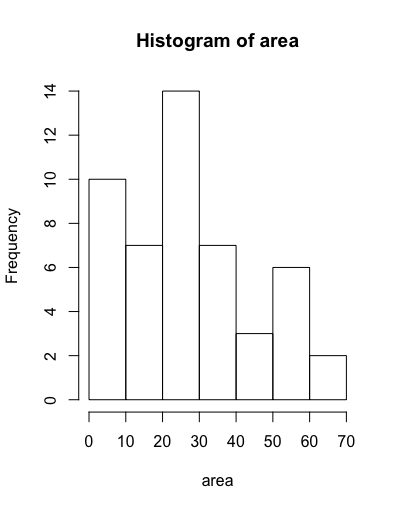
\includegraphics[scale=0.5]{images/areahist.png}
		\end{center}\par
		From this, we can once again conclude that the data is approximately symmetric.\par
		
	\part{b}
		\begin{center}
			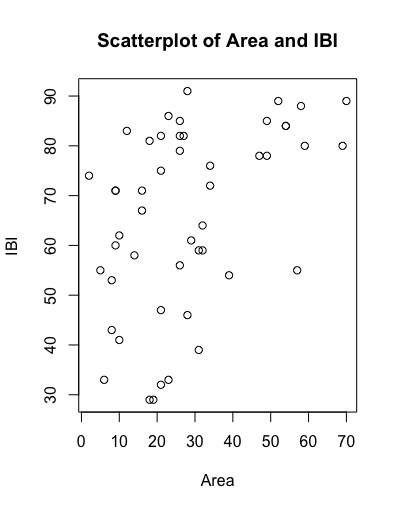
\includegraphics[scale=0.5]{images/areaibiscatter.png}
		\end{center}\par
		
		Based on the scatter plot, there is little association between the two variables as the points are scattered. No extreme outliers or observations are present in the sample either.\par
	
	\part{c}
		$IBI = \beta_{0} + \beta_{1}(Area) + \varepsilon_{i}, i = 1, 2, ... , 49$\par
	
	\part{d}
		$H_{0}:$ There is no linear association between the area and the IBI\par
		$\beta_{1} = 0$\par
		$H_{1}:$ There is a linear relationship between the area and the IBI\par
		$\beta_{1} \ne 0$\par
		
		After plugging in the function into R, the corresponding test statistic value is $t=3.415$ and the $p-value=0.00132$. Since the p-value is considerably small, we can reject $H_{0}$ stating that there is evidence of a linear relationship between the area and the IBI.\par
	
	\part{e}
		$IBI = 52.923 + 0.4602(Area)$\par
		$s=16.5346$\par
		Based on the above line and it's slope, for every one square meter of increment in the area, there will be 0.4602 units of increment in the IBI.\par
	
	\part{f}
		\begin{center}
			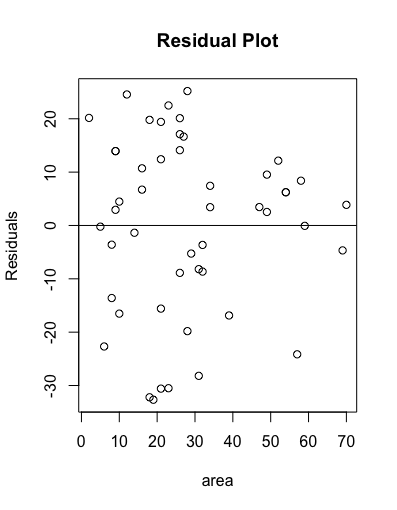
\includegraphics[scale=0.5]{images/resplot.png}
		\end{center}\par
		The observations are scattered over the origin line, and there is no pattern in the above plot. Therefore, the error are independent.\par
	
	\part{g}
		\begin{center}
			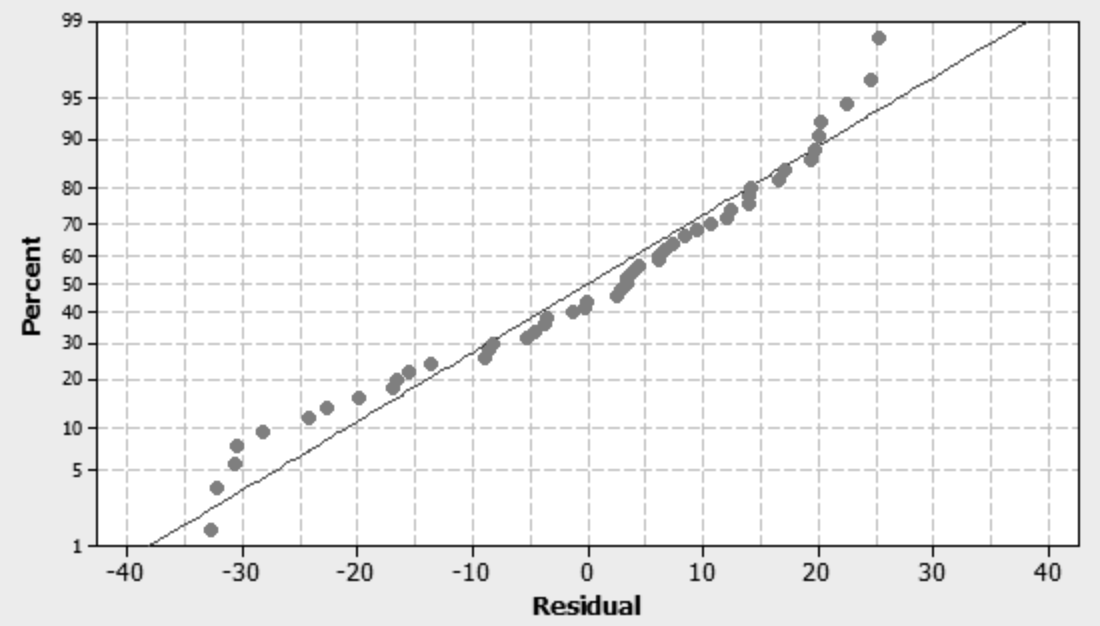
\includegraphics[scale=0.5]{images/ah.png}
		\end{center}\par
		The residuals are close to the line with no outliers in the sample. Therefore, the residuals are normal.\par
	
	\part{h}
		No violations of any assumptions of regression based on the scatterplot.\par
	

\question{10.33}{Pages 606 - 607}
	\part{a}
		Numerical data for IBI:\par
		
		\begin{center}
		\begin{tabular}{cccccccc}
			n & Mean & St. Deviation & Minimum & Q1 & Median & Q3 & Maximum\\
			49 & 65.94 & 18.28 & 29 & 54.50 & 71 & 82 & 91\\
		\end{tabular}\par
		\end{center}
		
		\begin{center}
			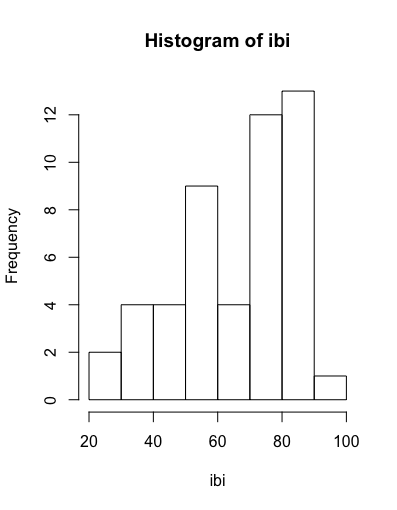
\includegraphics[scale=0.5]{images/ibihist.png}
		\end{center}\par
		Based on this, it is left-skewed.\par
		
		Numerical data for forest percent:\par
		
		\begin{center}
		\begin{tabular}{cccccccc}
			n & Mean & St. Deviation & Minimum & Q1 & Median & Q3 & Maximum\\
			49 & 39.39 & 32.2 & 0 & 10 & 33 & 63 & 100\\
		\end{tabular}\par
		\end{center}

		\begin{center}
			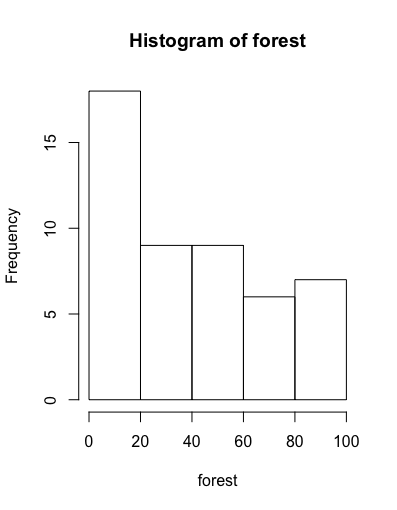
\includegraphics[scale=0.5]{images/foresthist.png}
		\end{center}\par
		Based on this, it is right-skewed.\par
		
	\part{b}
		\begin{center}
			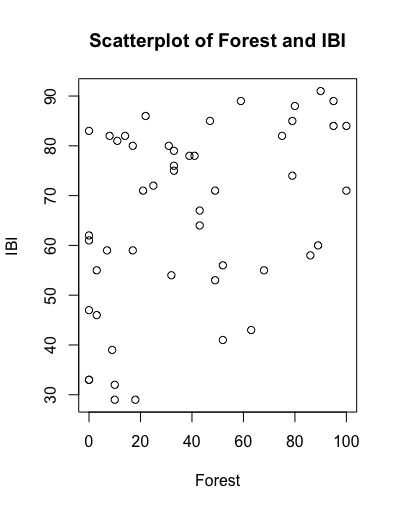
\includegraphics[scale=0.5]{images/forestibiscatter.png}
		\end{center}\par
		Based on this, the sample does not form any specific pattern, yet the IBI scatters more with smaller percentage values of forest and it tends upwards leading to the conclusion that they do not follow any specific pattern, but the relationship is weak and positive.\par
		
	\part{c}
		x is forest which is explanatory variable\par
		y is IBI which is response variable\par
		$ y_{i} = \beta_{0} + \beta_{1}x_{i} + \varepsilon_{i}, i = 1, 2, ... , 49$ where $\varepsilon_{i}$ are independent $N(0, \sigma)$ variables.\par
	
	\part{d}
		$H_{0}: \beta_{1}=0$\par
		$H_{1}: \beta_{1} \ne 0$
		
	\part{e}
		$\hat{IBI}=59.90 + 0.153(Forest)$\par
		Standard error is 17.79\par
		When testing the hypotheses in part (d), the testing statistic $t=1.92$ and the $p-value=0.061$ which means the null hypotheses fails to be rejected stating that the slope coefficient $\beta_{1}$ is not significantly different from 0.\par
		
	\part{f}
		\begin{center}
			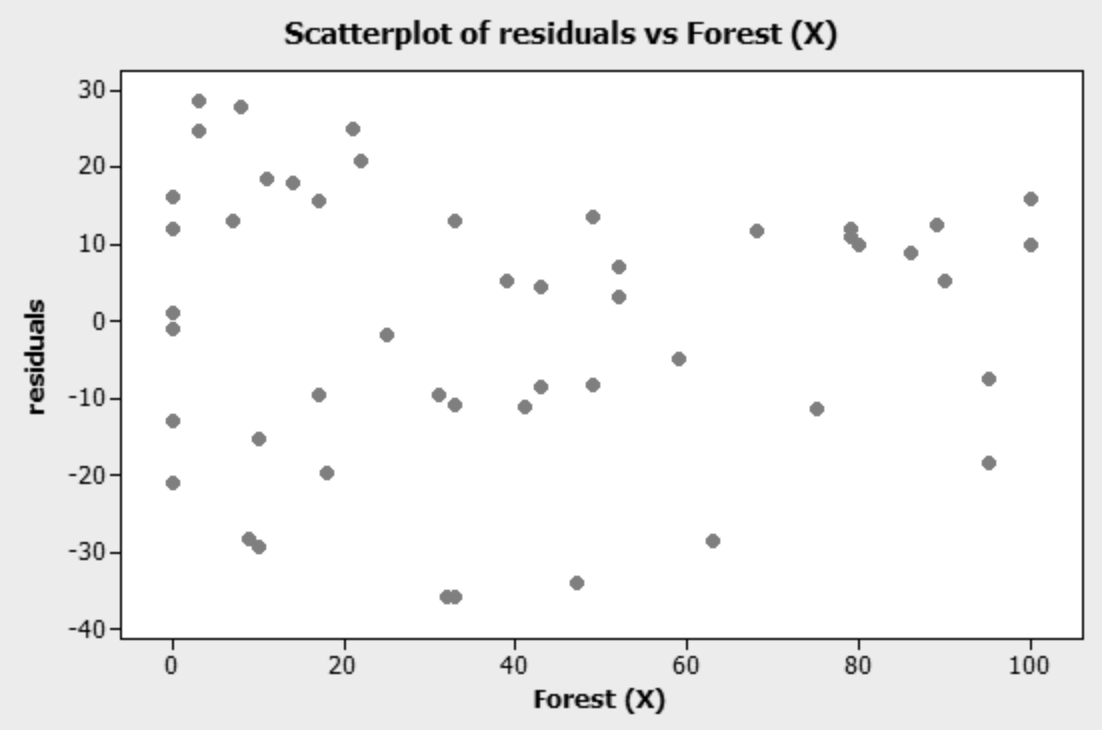
\includegraphics[scale=0.5]{images/ah2.png}
		\end{center}\par
		No pattern is observed here, the points are randomly scattered.\par
		
	\part{g}
		\begin{center}
			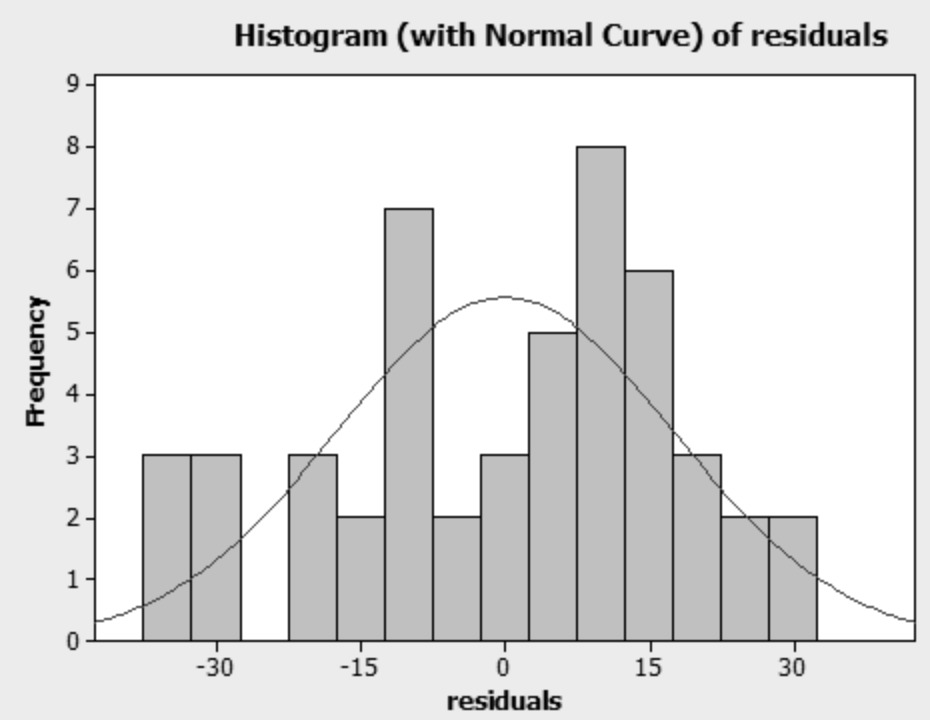
\includegraphics[scale=0.5]{images/ah3.png}
		\end{center}\par
		The residuals are left-skewed..\par
		
	\part{h}
		In part (c) it is assumed that the errors of the residuals are independent and $N(0, \sigma)$, but they are left-skewed as seen in part (g) therefore, the assumption is not reasonable.\par
		
		
\question{10.34}{Page 607}
	The Area as an explanatory variable is more desirable for the analysis because the $r^{2}$ value is greater while the $p-value$ is less, which is not the case for when the Forest is the explanatory variable.


\question{10.35}{Page 607}
	The first change ends up decreasing the $p-value$ which means the relationship becomes more significant because it amplifies the positive association between the two.\par
	The second change ends up increasing the $p-value$ which means the relationship is less significant, and it in turn weakens the association.\par

\question{10.36}{Page 607}
	\part{a}
		Using R, the regression line equation between IBI and the Area is: \par
		$IBI = 52.923 + 0.4602(Area)$\par
		The standard error is 16.5346\par
		The 95\% CI for 40 km$^{2}$ is (65.61, 77.04)\par
	
	\part{b}
		The 95\% PI for 40 km$^{2}$ is (37.58, 105.08)\par
	
	\part{c}
		Based on the CI in part (a), if one were to sample the number of streams, the expected average IBI would be between 65.61 km$^{2}$ and 77.04 km$^{2}$. From part (b), the expected IBI value corresponding to 40 km$^{2}$  watershed area would be between 37.58 km$^{2}$ and 105.08 km$^{2}$.\par
	
	\part{d}
		Yes because all of the assumptions of the regression study are assumed to be satisfiable in the available study. But that does not mean it should be applied to all streams in all states as there might be different factors that can influence the values such as geological location and other factors. The values of the intervals would be different for each state.

\question{10.37}{Page 607}
	$Area = 10, \hat{y} = 57.52$ but for $Forest = 63, \hat{y} = 69.55$.\par
	Both of the predictions though have uncertainty because the prediction intervals area about 70 units wide.\par
	

\end{document}